\subsection{Caso d'uso UC6: Ricerca e selezione questionario esistente}
\begin{center}
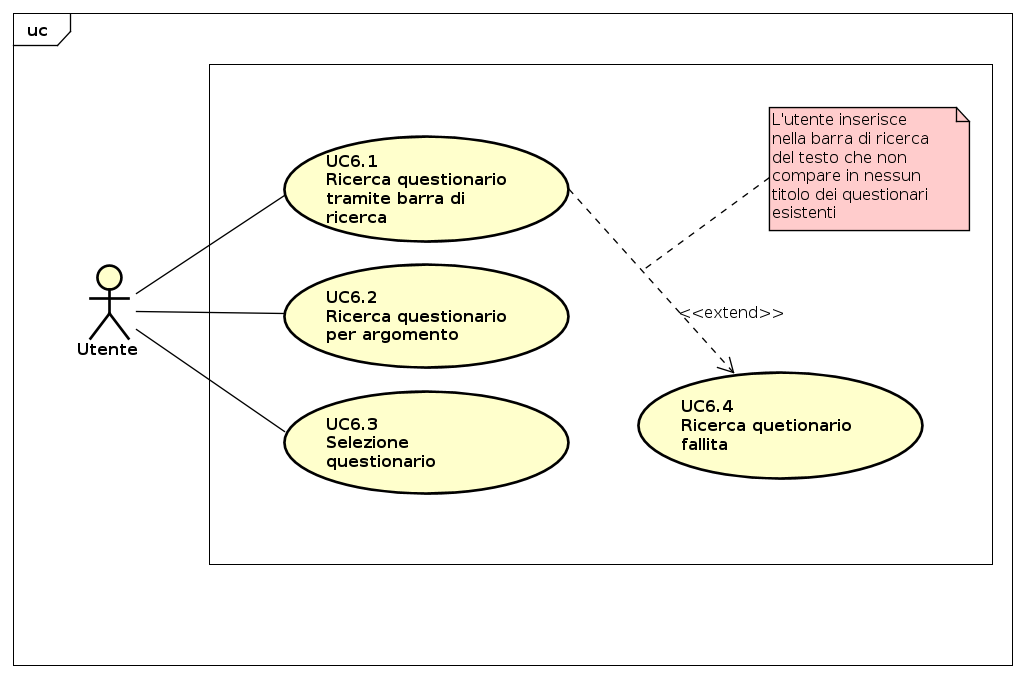
\includegraphics[scale=0.5]{UML/UC6.png}
\end{center}
\begin{itemize}
\item\textbf{Attori Principali}: Utente non autenticato, Utente autenticato, Utente autenticato pro;
\item\textbf{Descrizione}: nella schermata principale qualsiasi utente che voglia svolgere un questionario potrà ricercarlo attraverso:
\begin{itemize}
\item la barra di ricerca tramite il titolo del questionario;
\item una suddivisione per argomento dei questionari esistenti.
\\Per poterlo compilare dovrà poi selezionare il questionario che ha scelto.
\end{itemize}	
\item\textbf{Precondizione}: l'utente si trova nella pagina principale dell'applicazione;
\item\textbf{Postcondizione}: l'utente ha selezionato il questionario che vuole svolgere;
\item\textbf{Scenario principale}:
\begin{itemize}
\item L'utente cerca un questionario tramite barra di ricerca (UC6.1);
\item L'utente cerca un questionario per argomento (UC6.2);
\item L'utente seleziona il questionario scelto (UC6.3).
\end{itemize}
\item\textbf{Scenario alternativo}: L'utente inserisce nella barra di ricerca del testo che non compare in nessun titolo dei questionari esistenti;
\item\textbf{Estensioni}: Ricerca questionario fallita (UC6.4).
\end{itemize}

\subsection{Caso d'uso UC6.1: Ricerca questionario tramite barra di ricerca}
\begin{itemize}
\item\textbf{Attori Principali}: Utente non autenticato, Utente autenticato, Utente autenticato pro;
\item\textbf{Descrizione}: all'interno della pagina principale dell'applicazione è presente una barra di ricerca dove è possibile cercare, attraverso il titolo, un determinato questionario;
\item\textbf{Precondizione}: l'utente si trova nella pagina principale dell'applicazione;
\item\textbf{Postcondizione}: l'utente visualizza i questionari che hanno nel titolo il testo che ha scritto nella barra di ricerca;
\end{itemize}
\item\textbf{Scenario principale}: l'utente utilizza la barra di ricerca per cercare un questionario del quale conosce il titolo o parte di questo;
\end{itemize}

\subsection{Caso d'uso UC6.2: Ricerca questionario per argomento}
\begin{itemize}
\item\textbf{Attori Principali}: Utente non autenticato, Utente autenticato, Utente autenticato pro;
\item\textbf{Descrizione}: all'interno della pagina principale dell'applicazione è presente una sezione contenete tutti i questionari esistenti suddivisi per argomento trattato;
\item\textbf{Precondizione}: l'utente si trova nella pagina principale dell'applicazione;
\item\textbf{Postcondizione}: l'utente visualizza un insieme di questionari suddivisi per argomento;
\item\textbf{Scenario principale}: l'utente che non conosce i questionari esistenti, si reca nella sezione in cui sono suddivisi per argomento in modo da rendere più facile la scelta di uno di questi. 
\end{itemize}

\subsection{Caso d'uso UC6.3: Selezione questionario}
\begin{itemize}
\item\textbf{Attori Principali}: Utente non autenticato, Utente autenticato, Utente autenticato pro;
\item\textbf{Descrizione}: l'utente dopo aver scelto un questionario, per iniziare a compilarlo, deve selezionarlo;
\item\textbf{Precondizione}: l'utente ha scelto il questionario che vuole svolgere;
\item\textbf{Postcondizione}: l'utente ha selezionato il questionario scelto;
\item\textbf{Scenario principale}: l'utente seleziona il questionario che vuole iniziare a compilare.
\end{itemize}

\subsection{Caso d'uso UC6.4: Ricerca questionario fallita}
\begin{itemize}
\item\textbf{Attori Principali}: Utente non autenticato, Utente autenticato, Utente autenticato pro;
\item\textbf{Descrizione}: L'utente ha inserito nella barra di ricerca del testo che non compare in nessun titolo dei questionari esistenti;
\item\textbf{Precondizione}: l'utente ha utilizzato la barra di ricerca per cercare un questionario che non esiste;
\item\textbf{Postcondizione}: il sistema avvisa l'utente dell'errore verificatosi tramite un opportuno messaggio;
\item\textbf{Scenario principale}: l'utente visualizza un messaggio che lo avvisa del mancato ritrovamento di questionari;
\end{itemize}